% Horizon penetrating coordinates (vs. Schwarzschild coordinates)
% for a black hole spacetime, with excision
% Author: Jonah Miller
\documentclass[tikz,border=6pt]{standalone}
\usepackage{tikz}
\usetikzlibrary{arrows}
\usetikzlibrary{arrows.meta}
\usetikzlibrary{decorations.markings}
\usepackage{pgfplots}
\usepackage{amsmath}

\usepgfplotslibrary{fillbetween}

%\tikzset{>={Latex[length=3mm]}}

\tikzstyle{mybox} = [draw=black,
    rectangle, inner sep=10pt, inner ysep=10pt]
\tikzstyle{fancytitle} =[fill=blue!30, text=black]

\begin{document}
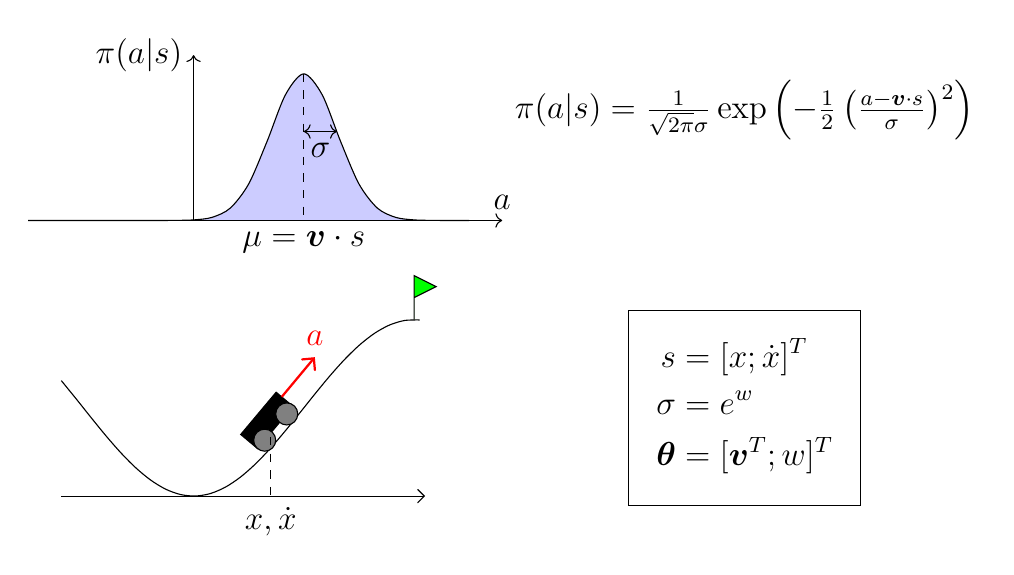
\begin{tikzpicture}[scale=1.4]
\large
\def\flagheight{4/5}
\def\carlength{0.2}

\draw[scale=1,domain=0.8:4.05,smooth,variable=\x] plot ({\x},{\flagheight*cos(90*\x)});

\def\mum{3}
\def\sigmam{0.3}

\def\heightfrommc{1.7}

%\draw[fill=blue!20,draw=blue!20] ({\mum - \sigmam},{\heightfrommc}) rectangle ({\mum+\sigmam},{\heightfrommc+1/(sqrt(2*3.14) * (\sigmam)) * e^(-1/2 * ((\sigmam )/(\sigmam))^2)});

\draw[fill=blue!20,scale=1,domain=0.5:4.5,smooth,variable=\x] plot ({\x},{\heightfrommc+1/(sqrt(2*3.14) * (\sigmam)) * e^(-1/2 * ((\x - \mum)/(\sigmam))^2)});


%\draw[scale=1,domain={\mum-\sigmam}:{\mum+\sigmam},smooth,variable=\x, fill=blue!20] plot ({\x},{\heightfrommc+1/(sqrt(2*3.14) * (\sigmam)) * e^(-1/2 * ((\x - \mum)/(\sigmam))^2)});



\draw[->] (2,\heightfrommc) -- (2,{\heightfrommc + 1.5}) node[left]{$\pi(a|s)$};
\draw[->] (0.5,\heightfrommc) -- (4.8,\heightfrommc) node[above]{$a$};
\draw[dashed] ({\mum}, {\heightfrommc+1/(sqrt(2*3.14) * (\sigmam))}) -- ({\mum}, \heightfrommc) node[below]{$\mu = \boldsymbol{v} \cdot s$};
\draw[<->] ({\mum}, {\heightfrommc+1/(sqrt(2*3.14) * (\sigmam)) * e^(-1/2 * ((\sigmam)/(\sigmam))^2)}) -- ({\mum+\sigmam}, {\heightfrommc+1/(sqrt(2*3.14) * (\sigmam)) * e^(-1/2 * ((\sigmam )/(\sigmam))^2)}) node[below, midway]{$\sigma$};


\def\columnwidth{7}
\draw[] (\columnwidth,\heightfrommc + 1) node{\large $\pi(a|s) = \frac{1}{\sqrt{2\pi}\sigma}\exp\left( -\frac{1}{2}\left(\frac{a-\boldsymbol{v}\cdot{s}}{\sigma}\right)^2 \right)$};

\node[mybox](box) at ({\columnwidth}, 0){\large $\begin{aligned} s &= [x ; \dot{x}]^T \\ \sigma &= e^w \\ \boldsymbol{\theta} &= [\boldsymbol{v}^T; w]^T\end{aligned}$};
%\node[fancytitle] at (box.north) {saf};

\draw[-,fill=green] (4,\flagheight) -- (4,{\flagheight + 0.4}) -- (4.2,{\flagheight + 0.3}) -- (4,{\flagheight+0.2});


\def\carx{2.7}
\def\cary{\flagheight*cos(90*\carx)}
\def\carytwo{\flagheight*cos(90*(\carx+\carlength))}

\def\deltax{-0.055}
\def\deltay{0.07}

\draw[-,fill=black,rotate around={50:({\carx+\deltax},{\cary+\deltay})}] ({\carx+\deltax-0.1},{\cary+\deltay}) rectangle({\carx+\deltax+0.4},{\cary+\deltay+0.2});
\draw[-,fill=gray] ({\carx+\deltax},{\cary+\deltay}) circle(0.1);
\draw[-,fill=gray] ({\carx+\carlength+\deltax},{\carytwo+\deltay}) circle(0.1);

\draw[thick, red, -angle 90] (2.8,0.1) -- (3.1,0.46) node[above]{$a$};

%\draw[red](2,1) node{$r=-F^2$};

%\draw[-angle 90,thick] (0.8,{-\flagheight}) -- (4.1,{-\flagheight}) node[above=6pt,left=0.5pt]{$x$};

\draw[-angle 90] (0.8,{-\flagheight}) -- (4.1,{-\flagheight});% node[above]{$x$};
\draw[dashed] ({\carx},{\cary+0.4}) -- ({\carx}, {-\flagheight}) node[below]{$x, \dot{x}$};

\end{tikzpicture}
\end{document}